% Start - Hardware/Control Unit/Reset
%write Between the comments

\subsubsection{Reset}

	\paragraph{Reset}
	logic is used to set the \gls{mcu} in known state.The reset circuit for this \gls{mcu} is provided in figure \ref{fig:reset_circuit}.(cite avr042 here)
	
	\begin{figure}[H]
		\caption{Reset Circuit}
		\label{fig:reset_circuit}
		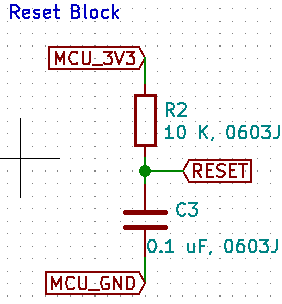
\includegraphics[scale=1]{reset_ckt.png}
	\end{figure}
	
	\textbf{Value Calculation}	
	\paragraph{R2}
	is acting as pull-up resistor here, which is used for high voltage programming (10V - 12V). Recommended value of pull-up resistor is 10 K$\Omega$.
	
	\paragraph{C3} 
	is used to filter high frequency noise, typical value is 100 nF (or 0.1 $\mu$F).
	
	\textbf{Power Calculation}
	
	Maximum allowable voltage for $V_{cc}$ is 5.5 V and $ V_{thresh}$ for reset pin detection is 1.1 V (cite datasheet here). 
	\begin{itemize}
		\item[R1:]
			\begin{align}
				n =m
			\end{align}
	\end{itemize}
	
%http://www.ti.com/interface/circuit-protection/esd-protection-and-tvs-surge-diodes/support-training.html
% End - Hardware/Control Unit/Reset